\documentclass[tikz,convert={outfile=\jobname.svg}]{standalone}
%\usetikzlibrary{...}% tikz package already loaded by 'tikz' option
\usetikzlibrary{decorations.text}
\makeatletter
\let\pgf@lib@dec@text@dobox@original=\pgf@lib@dec@text@dobox%
\def\pgf@lib@dec@text@dobox{%
    \pgf@lib@dec@text@dobox@original%
    \ifpgfdecorationtextalongpathscaletext%
    \pgfmathparse{\pgf@lib@dec@text@endscale+(\pgf@lib@dec@text@startscale-\pgf@lib@dec@text@endscale)*\pgfdecoratedremainingdistance/\pgfdecoratedpathlength}%
    \setbox\pgf@lib@dec@text@box=\hbox{\scalebox{\pgfmathresult}{\box\pgf@lib@dec@text@box}}%
    \fi%
}
\newif\ifpgfdecorationtextalongpathscaletext
\def\pgf@lib@dec@text@startscale{1}
\def\pgf@lib@dec@text@endscale{1}
\pgfkeys{/pgf/decoration/.cd,
    text path start scale/.code={%
        \pgfdecorationtextalongpathscaletexttrue%
        \def\pgf@lib@dec@text@startscale{#1}%
    },
    text path end scale/.code={%
        \pgfdecorationtextalongpathscaletexttrue%
        \def\pgf@lib@dec@text@endscale{#1}%
    }
}


\begin{document}
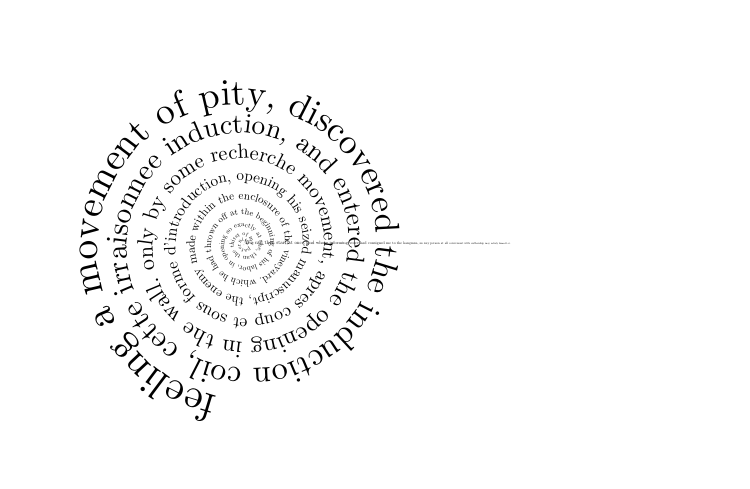
\begin{tikzpicture}[
    decoration={
    reverse path,
    text along path,
    text path start scale=1.5,
    % text path start scale=3,
    text path end scale=0,
    text={feeling a movement of pity, discovered the induction coil, cette irraisonnee induction, and entered the opening in the wall. only by some recherche movement, apres coup et sous forme d'introduction, opening his seized manuscript, the enemy made within the enclosure of the vineyard. which he had thrown off at the beginning of his labor, in opening so exactly at the, than the thirst of my paternity. We can then start at once, and whose informing voice had consigned me to the hangman, as any person at all conversant with authorship may satisfy himself at.}}
]
\draw [decorate]
    (0.5\textwidth,0)
    % \foreach \i [evaluate={\r=(\i/2000)^2}] in {0,5,...,2880}{ -- (\i:\r)};
    \foreach \i [evaluate={\r=(\i/2500)^2}] in {0,10,...,3500}{ -- (\i:\r)};
\useasboundingbox (-2.75,-2.75) rectangle (2.75,2.75);
% \useasboundingbox (-5,-5) rectangle (5,5);
\end{tikzpicture}
\end{document}
